\subsection{Четвёртый этап. Точная временная синхронизация и эквалайзинг}

Данный этап посвящён борьбе с искажениями, вносимыми многолучевым распространением сигнала (см. раздел 3.b.ii), а также окончательной временной синхронизации.

\begin{figure}[h!]
\centering
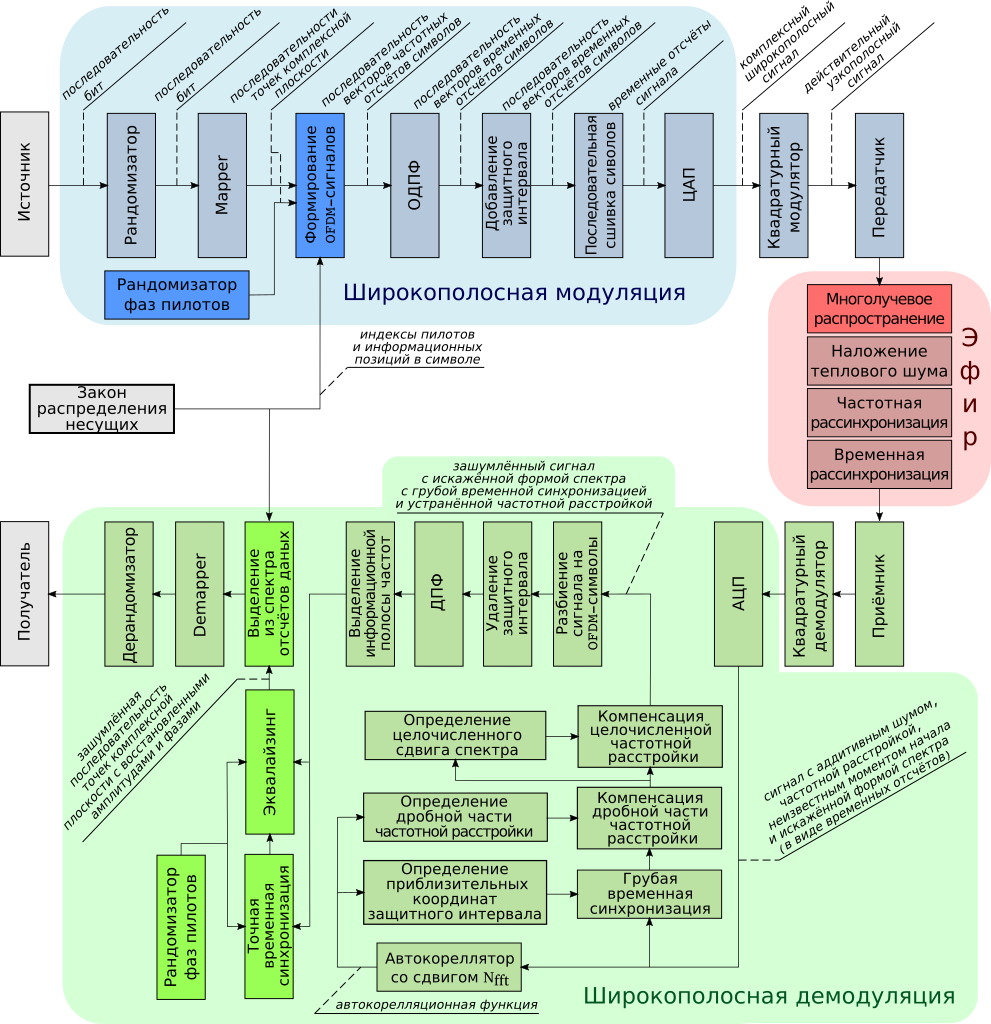
\includegraphics[width=1\textwidth]{OFDM-4.png}
\caption{Схема модели на четвёртом этапе} \label{fg:schem3}
\end{figure}

\subsubsection{Передающая сторона}
Ключевым элементом этапа являются пилотные несущие (3.C.c). В первом приближении их распределение в информационной части спектра символов постоянно и не меняется от символа к символу. В таком случае распределение пилотов задаётся параметром \textit{amount\underline{ }ratio\underline{ }pilots} -- долей  пилотных несущих. Эти несущие необходимо распределить максимально равномерно среди полного количества несущих \textit{n\underline{ }carriers} символа, причём первая и последняя поднесущие обязательно должны быть пилотными.

Амплитуды пилотных несущих должны превышать наибольшие амплитуды точек созвездия. Это отношение устанавливается параметром $amp\_ratio\_pilots>1$. его рекомендуемое значение составляет $\dfrac{4}{3}$. 

%%Описать в п.5 либо дать описание здесь, в том числе про пик-фактор
Фазы пилотов в первом приближении можно принять одинаковыми, нулевыми. Как рассмотрено в п.5, периодическое распределение информационных отсчётов в спектре приводило к возрастанию пик-фактора. Точно таким же образом дело обстоит с пилотными отсчётами. Дело осложняется тем, что пилотные несущие передаются на повышенной амплитуде и влияние их на пик-фактор велико. Введение рандомизатора, позволяющего разбить периодичность распределения фазы пилотов, помогает снизить пик-фактор. Обычно для построения последовательности комплексных амплитуд несущих используется созвездие \textit{BPSK} с повышенной амплитудой, на вход которого подаётся псевдослучайная битовая последовательность. В таком случае система приобретает ещё один параметр -- \textit{initreg\underline{ }pilot} -- начальное состояние регистра сдвига ГПСЧ рандомизатора битовой последовательности для пилотов.

Наиболее удобный способ работы с информационными и пилотными поднесущими символа -- индексация информационных точек и пилотов. Для этого создаются две соответствующих строки номеров упомянутых позиций в информационной части спектра.

\subsubsection{Канал}

Единственный фактор, вводимый на данном этапе -- многолучевое распространение. Для двух заданных массивов параметров $t\_copies>0$ и $-1<c\_copies<1$ на сигнал накладываются его повторённые копии c задержками $t\_copies[k]$ и весами $с\_copies[k]$.

\subsubsection{Принимающая сторона}

После выделения информационной части спектра символа  производятся точная временная синхронизация и эквалайзинг (4.b), затем из спектра выделяются значения, соответствующие информационным точкам. 

Оба восстанавливающих блока работают по схеме определения искажений по фазе и амплитуде пилотных несущих, что возможно, поскольку исходные фазы и амплитуды известны и приёмнику, и передатчику. Затем производится интерполяция этих отклонений на информационные позиции спектра символа. Метод интерполяции устанавливается параметром \textit{int\underline{ }method}. Рассматриваются линейная интерполяция и интерполяция кубическим сплайном.

\subsubsection{Вопросы и задания}
\begin{enumerate}
\item
Научиться генерировать массивы для индексации информационных и пилотных точек спектра для заданных общего количества несущих и доли пилотных несущих. Внедрить в символ постоянные пилотные несущие нулевой фазы на передающей стороне и извлекать информационные точки на принимающей стороне.
\item
Вычислить пропусную способность системы (в количестве исходных информационных бит на OFDM-символ) для заданной доли пилотных несущих в символе.
\item
Смоделировать эффект многолучевого распространения, наложив набор копий сигнала, задаваемый массивами \textit{t\underline{ }copies} и \textit{c\underline{ }copies}. Построить модуль ДПФ  информационной части символа после её выделения, а также получаемое созвездие.
\item
Реализовать эквалайзинг и точную временную синхронизацию для методов линейной и сплайновой интерполяции. Построить графики интерполированной ошибки по фазе информационной части спектра и интерполированной относительной ошибки по амплитуде. Построить модуль ДПФ информационной части символа и получаемое созвездие. Убедиться, что восстановление происходит.
\item 
Ввести рандомизацию комплексных амплитуд пилотных несущих. Использовать созвездие \textit{BPSK} на повышенной амплитуде $amp\_ratio\_pilots$. Регистр сдвига ГПСЧ инициализировать вектором \textit{initreg\underline{ }pilot}. Вычислить пик-фактор для сигнала без рандомизации пилотов и с ней.
\item %%описать в разделе задание двумерной маски через Dx и Dy
Ввести двумерную маску пилотов, задаваемую двумя параметрами -- интервалами  \textit{Dx} и \textit{Dy} (см раздел 2.C.c). Теперь распределение пилотных несущих от символа к символу будет меняться. В качестве опорных значений при интерполяции теперь берутся все пилоты текущего символа, а также все, кроме крайних, пилоты $Dy-1$ соседних с ним символов.

Стоит отметить, что несмотря на двумерность маски пилотов, интерполяция остаётся в этом случае одномерной. Такой подход позволяет, с одной стороны, сэкономить на количестве пилотов, увеличивая количество информационных позиций (и, соответственно, пропускную способность) при фиксироанном периоде их следования в спектре, с другой -- максимально равномерно распределить заданное количество пилотов во временной и частотной областях. Кроме того, эта схема более гибко обрабатывает изменения во времени характеристик системы (задержек и амплитуд лучей, доплеровских смещений, частотной расстройки).
\end{enumerate}